\documentclass[12pt,a4paper,twocolumn]{article}
\usepackage[latin1]{inputenc}
\usepackage{amsmath}
\usepackage{amsfonts}
\usepackage{amssymb}
\usepackage{textcomp}
\usepackage{graphicx} 
\author{Alexandros-Panagiotis Oikonomou}
\title{Image Contour Extraction}
\begin{document}
\maketitle
\newpage
\thispagestyle{empty}
\mbox{}
\newpage
\thispagestyle{empty}
\mbox{}
\newpage
\thispagestyle{empty}
\mbox{}
\section{Introduction}
For the assignment of the Intelligent Algorithms course I was asked to implement an Image Contour Extractor algorithm. With the use of MATLAB the principle of Dynamic Programming was adopted for the implementation. Throughout this report the design of the algorithm is documented along with findings made by testing the algorithm. 
\section{Program Design}
This section will describe the design principles used to implement the algorithm.
\subsection{Search Space}
The design to extract the search space has been kept into a fairly simple level. There exists a function search\_space which takes as arguments the image matrix returned by the imread command and the contour initialisation matrices. It returns a 3D Matrix of type (rows(image),M,3) called points. M is the number of rows the user wishes to have in the search space. In the first index of the third dimension (i,j,1) the x value of the image is stored, in the second index (i,j,2) the y value of the image is stored and in the third index (i,j,3) the intensity of the (x,y) point is stored. That way each (i,j) point in the points matrix corresponds to an (x,y) value of the image. Before the matrix is returned the values of the intensities are negated.
\subsection{Dynamic Programming}
In order to apply the algorithm supplied in the assignment there exists a function get\_energies which takes as arguments the image matrix, the two initialisation contours and the $\lambda$ that the user wishes. The first command is to call the search space function mentioned above. As output parameters it returns an energy matrix, a position matrix and the matrix returned by the search space now renamed intensity. The intensity matrix is returned to be used for backtracking. The energy matrix is a 3D matrix of the form (rows(intensity),columns(intensity),rows(intensity)).
The first two terms correspond to the same points as in the intensity matrix. 

Depending on the point the algorithm is currently at, the minimum energy of all the points in the previous column is stored in the last dimension of the energy matrix.The reason this the dimension is a vector of size rows(intensity) is that the above action is done for all the points of the next column. The energy is computed according to (1). 
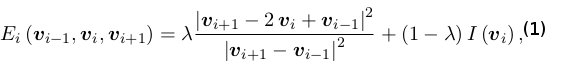
\includegraphics[width=250pt,height=50pt,scale=1]{energy_eq.jpg}
The position matrix has the same first two terms, but the difference is that in the third term, the row where the minimum energy was found is stored, instead of the value itself. The result of computing energies and position matrices for all these points is that a quadruple for-loop is used
\subsection{Backtracking}
The backtracking is completed in a function called get\_contour which returns the points of the contour. The initial calculations of this function locate the minimum energy in all the vectors of the next to last column of the search space along with its row and depth index. The reason this column is picked is that in the last column the computation is not completed in its entirety, due to the fact that there is no next column to do the computation correctly(1). The algorithm now jumps to the node with the row index and the depth index returned in the previous calculation and reads the value in the position matrix. Then the optimal path is chosen, by going to the next column and selecting the row from the value in the position matrix. The depth is found from the index the depth of the minimum energy value was found.
\subsection{Negating Images}
It is also noteworthy to mention that the intensities of the points are negated before passed on to the produce\_energies function. The reason for that is that the algorithm searches and stores the minimum energy. That means that lower intensities are desired for the optimisation. The problem with the returned image, when applying the imread function, is that blacker pixels have lower intensities and whiter pixels have higher intensities. By negating the intensities, this property is reversed and hence the algorithm searches for pixels which seem whiter. Negating the image is done by the function negating\_intensities.
\section{Algorithm Testing}
This section will report the findings of applying the algorithm in different situations.
\subsection{Initial Results}
The initial test of the algorithm was to be done in a picture supplied in the assignment specification. The testing configuration asked was to be with $\lambda$=0.5. However M was not specified and so M=100 was chosen arbitrarily. The result contour displayed all but one points to lie perfectly on the outline of the tongue(5.1 Appendix).
\subsection{Scalability with changes in M}
For every point in a column the energies of all the points of the previous column need to be computed. That must also be done for each of the points of the next column. So for one column there are M$^3$ operations. 
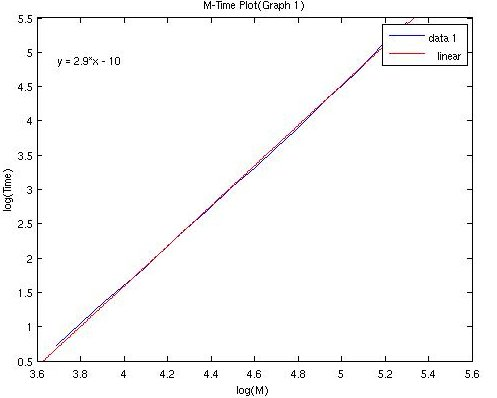
\includegraphics[width=250pt,height=200pt,scale=1]{logs.jpg}	
More explicitly for the entirety of the search space there must be N*M$^3$ operations, where N is the number of columns of the search space. The logarithms in Graph 1(Appendix 5.4) are taken in order to compute the exponent of the polynomial. In this case it is found to be a=2.9. This almost matches the theory explained above. The reason why it does not match perfectly can be attributed to machine irregularities.
\subsection{Robustness with changes in Lambda}
Changing $\lambda$ seemed to make the contour behave differently on certain occasions. 
It was observed that for 0.1 $<$ $\lambda$ $<$0.7 the contour did not seem to change significantly. It remained the same as it was for $\lambda$=0.5(Appendix 5.1).
On the contrary for 0.8 $<$ $\lambda$ $<$0.9 it was observed that this point would now lie in the tongue, adjacent with the rest of the contour points. This made the contour more precise and accurate(5.2.1 Appendix).
Finally, a configuration with $\lambda$'=0.00001 was tested. Again most of the points lied on the tongue, but this time in addition to the one irregular point that existed in previous $\lambda$ tests, there were some additional irregular points in the initial points of the contour(5.2.2 Appendix). This can be attributed to the fact that with low $\lambda$'s emphasis is given in the intensity of the points and the intensity is found high at these points.
\subsection{Different contour initialisations}
To identify the strength of the algorithm, different initialisations of contours were tested.
Firstly a contour with higher top initial contour was tested(5.3.1 Appendix) and it was verified that the final contour would still be correctly drawn. The reason for that was that the intensities of the added search space were more or less the same as before. Next a lower bottom initial contour was chosen(Appendix 5.3.2). This time it is apparent that the contour breaks badly, even though some points still lie in the tongue outline. The reason for that is that points above the new initial bottom contour have lower intensities than those that lie on the tongue. That forces the algorithm to store their energies in the energy matrix, instead of the ones that lie on the tongue. A final initialisation of the bottom initial contour was tested, by having its initial x-points move to the right by 50, relative to the x-axis(Appendix 5.3.3). It is noticeable that in the lower X's, the contour breaks. The reason for that is that the lower X's of the bottom initial contour do not have access to the X's located in the tongue, which makes the energy calculation break and calculate unrealistic distance values.
\subsection{Other tested images}
In order to test the algorithm in a different environment, it was run with another image.(Appendix 5.5). Some points of the contour seem to lie in the stick, but since the stick seems to have 2 distinctly different dimensions it is hard for the algorithm to locate the contour. In addition, towards the right end of the stick the background of the stick seems to have high intensity.
\section{Conclusion}
The Image Contour algorithm was proved to be effective and robust both in the initial testing phase and with changes made in $\lambda$ values, when testing with the picture of the tongue. It also seemed effective when testing with different contour initialisation, as long as the the contours were not destructive to its functionality. The scalability of the algorithm in theory matched the implementation as shown by running the algorithm with different M values. 

The algorithm seems to be strong as long as appropriate images are used. This was on display when running the algorithm in the image with the stick.

Improvements that could be done in this piece of course work, would be removing some of the four for-loops and making them implicit and done by MATLAB internally in order to increase performance. Closed contours could also be implemented in order to produce contours for images with distinct dimensions and filling inside, such as the aforementioned image.

\newpage
\mbox{}
\newpage
\mbox{}
\section{Appendix}
\subsection{Initial result}
$\lambda=0.5$ and M=100
\newline
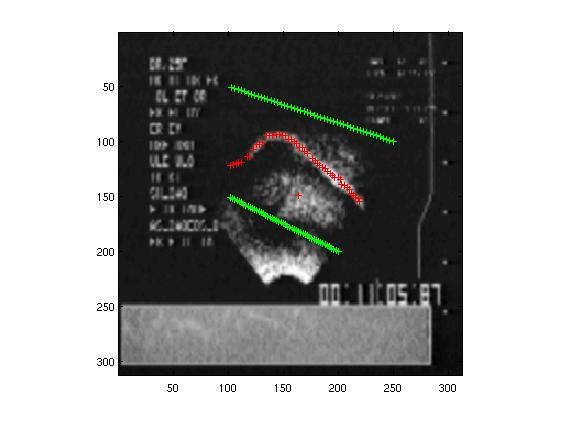
\includegraphics[width=500pt,height=400pt,scale=1]{points_1_to_7.jpg}
\newpage
\mbox{}
\newpage

\subsection{Tweaking $\lambda$'s}
\subsubsection{High $\lambda$'s}
0.8$<$ $\lambda$ $<$0.9 and M=100
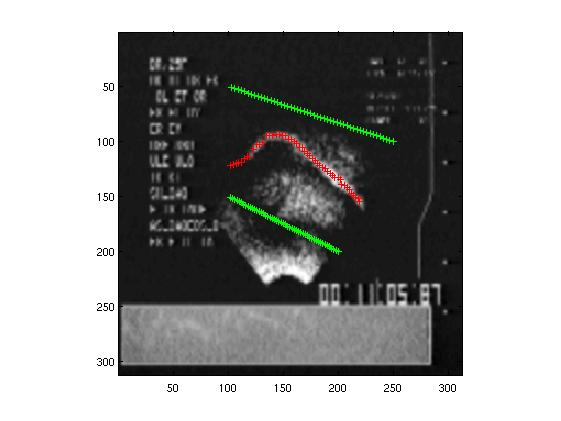
\includegraphics[width=500pt,height=400pt,scale=1]{89.jpg}
\newpage
\mbox{}
\newpage
\subsubsection{Low $\lambda$'s}
$\lambda$=0.00001 and M=100
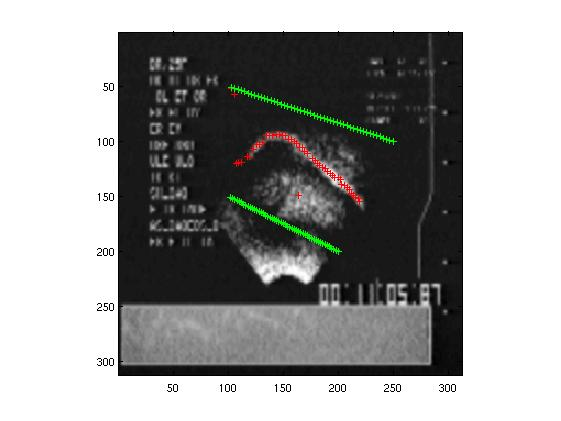
\includegraphics[width=500pt,height=400pt,scale=1]{small_values.jpg}
\newpage
\mbox{}
\newpage
\subsection{Contour initialisations}
\subsubsection{Higher Top Initial Contour}
The y of the top contour is decreased by 50.
$\lambda$=0.8 and M=100
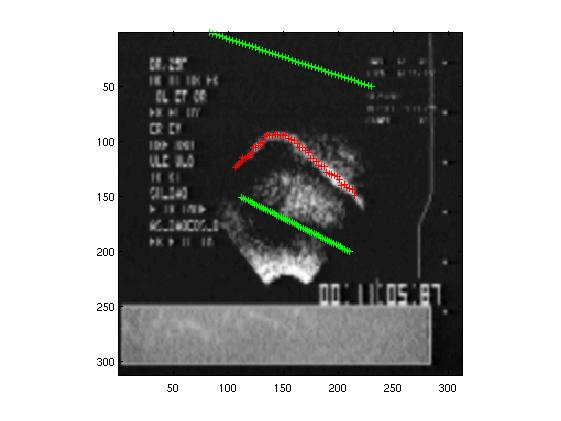
\includegraphics[width=500pt,height=400pt,scale=1]{top_plus_many.jpg}
\newpage
\mbox{}
\newpage
\mbox{}
\subsubsection{Lower Bottom Initial Contour}
The y of the top contour is decreased by 50.
$\lambda$=0.8 and M=100
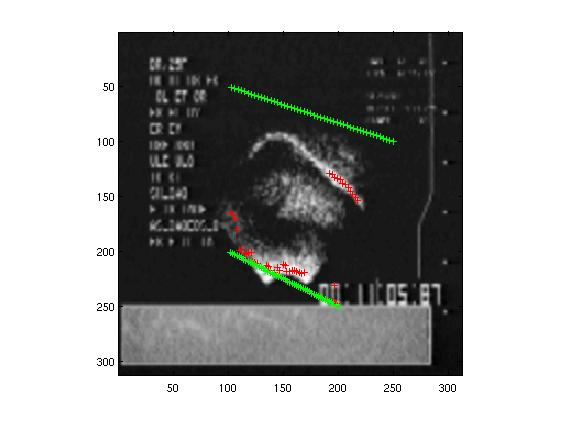
\includegraphics[width=500pt,height=400pt,scale=1]{bot_plus_50.jpg}	
\newpage
\mbox{}
\newpage
\mbox{}
\subsubsection{Bottom Initial Contour to the Right}
$\lambda$=0.8 and M=100
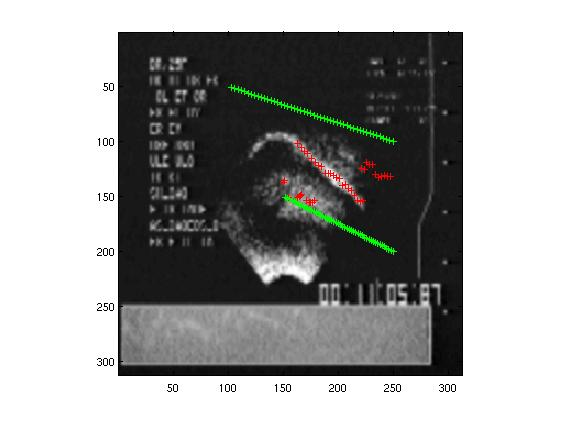
\includegraphics[width=500pt,height=400pt,scale=1]{bot_plus_50x.jpg}	
\newpage
\mbox{}
\newpage
\mbox{}
\subsection{Values for Graph 1}
The values of M used and the time results. To produce this table the tic-toc function was used in MATLAB. The values refer to Graph 1 in the text
\newline
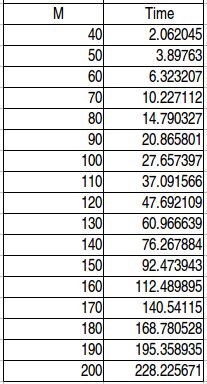
\includegraphics[width=150pt,height=350pt,scale=1]{table.png}	
\newpage
\mbox{}
\newpage
\mbox{}
\subsection{Stick Image}
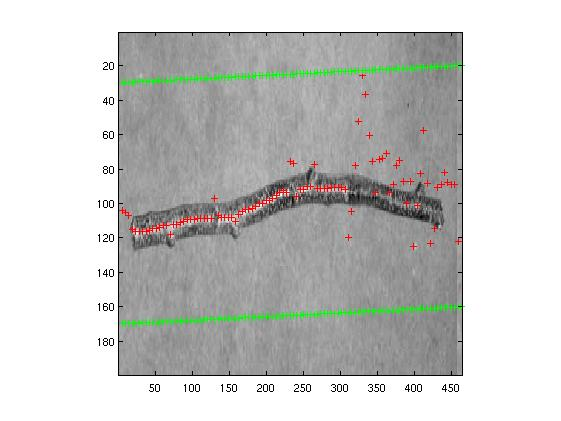
\includegraphics[width=500pt,height=400pt,scale=1]{stick_cont.jpg}	
\end{document}